
\chapter{Fundamentação Teórica\label{chap:FundamentacaoMatematica}}

% Resumo opcional. Comentar se não usar.
\resumodocapitulo{Opcional, geralmente se colocam pequenos resumos
ou citações que se achar relevantes.}


\section{Introdução}

Este capítulo irá apresentar algumas soluções para o problema de tomada de decisões em sistemas de robótica móvel encontradas em outros trabalhos anteriores nessa área. Será abordado, também, o problema de aprendizagem por reforço e algumas alternativas de como é executado na literatura. Por último, esse capítulo irá introduzir a teoria matemática por trás dos algoritmos utilizados nesse projeto.


\section{Revisão Bibliográfica}

Aqui iremos descrever diferentes abordagens encontradas na literatura para o problema de tomada de decisões aplicado a sistemas de robótica móvel. A tomada de decisões é um problema de amplo espectro para o qual existem várias estratégias diferentes que tentam solucioná-lo.

Analisando a literatura, podemos ver a preferência crescente por algoritmos probabilísticos nessa área, no lugar dos determinísticos. Isso provem da incerteza presente no mundo real, que deve ser modelada pelo algoritmo adotado. Para uma modelagem verdadeira e precisa do mundo real, é preciso considerar as incertezas presentes nele.

Muitos algoritmos de planejamento de tarefas são específicos para as tarefas que seus robôs irão desempenhar, alguns exemplos são na área de exploração, por exemplo, o uso de algoritmos de exploração de fronteiras [4, 5, 6] ou na área de braços robóticos para planejamento de manipulação de objetos para robôs com dois braços [7].

Para o nosso sistema queríamos um algoritmo que não fosse específico para um único tipo de aplicação. Analisando a literatura mais a fundo, vemos que muitos algoritmos nessa área são baseados na cadeia de Markov. Ela diz que o ambiente pode ser modelado por um número de variáveis de estado em que cada estado depende apenas do estado exatamente anterior ( $ P(S_t\mid S_{t-1}S_{t-2})=P(S_t\mid S_{t-1}) $ ), ou seja, o sistema não tem memória de longo prazo [8].

Um algoritmo baseado na cadeia de Markov que é muito utilizado é o Processos de Decisão de Markov (Markov Decision Processes, MDP) [3]. Um problema desse algoritmo é que, embora ele leve em conta que as ações executadas podem ter um comportamento imprevisível, ele não incorpora a incerteza provinda dos sensores. Em outras palavras ele considera que o estado do sistema pode ser completamente observado a todo instante, o que não é correto.

Um algoritmo que corrige esse problema é o Processos de Decisão de Markov Parcialmente Observável (Partially Observable Markov Decision Processes, POMDP) [3]. Esse algoritmo retorna para o caso geral completamente probabilístico em que ambos os sensores e os atuadores tem funcionamento imprevisível e com certa curva conhecida de probabilidade. O problema com esse algoritmo é a sua demanda computacional, mesmo podendo ser calculado off-line e salvo, ele muitas vezes não é computacionalmente possível.

Em [9] Pineau e Thrun utilizam uma estratégia de vários POMDPs hierarquizados para reduzir o problema de requisição computacional que um único POMDP combinado iria precisar.

Outra estratégia para o planejamento de tarefas é uma estratégia reativa baseada na seleção de comportamentos presente em [1, 10]. Essa é uma estratégia interessante, pois, computacionalmente ela é eficiente, ao se selecionar somente um comportamento e posteriormente se escolher uma ação para ele, consegue-se reduzir consideravelmente as opções a se tomar (existem menos comportamentos do que ações possíveis). Essa estratégia foi expandida posteriormente em [11] para se aprender a os modelos probabilísticos de seleção de comportamentos a partir de entradas humanas.

Na área de aprendizagem de modelos ou de políticas para execução de ações, existem vários algoritmos baseados no MDP citado acima. Alguns deles, que focam apenas na aprendizagem do modelo [refs Model learning] tem várias aplicações, sendo análise de mercados para economia uma delas [refs Model learning calvet]. Outro exemplo de algoritmo de aprendizagem é o de diferença temporal, que é utilizado para avaliar uma dada política [refs temporal difference, q learning book].

Outros algoritmos de aprendizagem por reforço permitem aprender uma política ótima de comportamentos ou ações para um dado agente. Um desses algoritmos é o Q Learning [refs q learning book, q learning], que é um algoritmo simples, mas eficiente, que aprende valores de ganho para cada par ação-estado, e com isso consegue alcançar uma política ótima. Outro é o ator crítico [refs reinforcement learning book, actor crictic], que aprende uma política ótima ao separa um ator, o qual escolhe essa política, e um crítico, que avalia a política e provê um feedback para o ator.

Nesse trabalho nós utilizaremos os algoritmos presentes em [1, 10] para fazer uma seleção de comportamento e ação para um agente móvel com sensores probabilísticos. Além disso, utilizaremos um algoritmo de aprendizagem por reforço, q learning, presente em [ref reinforcement learning book], para aprender uma política ótima de escolha de comportamento.


\section{Filtro Bayesiano}

Um filtro bayesiano é uma abordagem probabilística para estimar uma função de densidade de probabilidade desconhecida de forma recursiva no tempo, utilizando ações e observações além de um modelo matemático do processo.

No filtro bayesiano nós queremos obter a distribuição conjunta de probabilidade:

\begin{equation}
P ( M^{0: t} S^{0: t} Z^{0: t} \mid \pi_f )
\end{equation}

Sendo $ M^i $ o conjunto de ações no tempo $ i $, $ S^i $ o estado do sistema nesse instante e $ Z^i $ os dados dos sensores, também nesse instante. Essa função de probabilidade representa a probabilidade de uma sequência de ações, observações e estados acontecerem dado o que se sabe sobre o mundo. Para obter esse valor tiraremos proveito das propriedades desse sistema que é baseado numa cadeia de Markov.

\begin{equation}
        P ( M^{0: t} S^{0: t} Z^{0: t} \mid \pi_f ) = P ( M^0 S^0 Z^0 \mid \pi_f ) \cdot \prod\limits_{j =1}^{t} 
        \left(
            \begin{array}{l}
                P( S^j \mid S^{j -1} M^{j -1} \pi_f ) \\
                \times P( Z^j \mid S^j \pi_f ) \\
                \times P( M^j \mid S^j M^{j -1} \pi_f )
            \end{array}
        \right)
\end{equation}

Essa equação explicita quatro itens:

\begin{itemize}
  \item $ P \left( M^0 S^0 Z^0 \mid \pi_f \right) $ : As probabilidades do estado inicial do sistema são necessárias para se obter seus futuros valores;
  \item $ P \left( S^j \mid S^{j-1} M^{j-1} \pi_f \right) $ : Cada estado depende do estado anterior e de que ação foi tomada (termo de predição);
  \item $ P \left( Z^j \mid S^j \pi_f \right) $ : É necessário um modelo de probabilidades do sensor (termo de observação)
  \item $ P \left( M^j \mid S^j M^{j-1} \pi_f \right) $ : A escolha da próxima ação depende de qual o estado do sistema e qual a ação anterior (termo de decisão de ação)
\end{itemize}

Com essas densidades probabilísticas podemos decidir por estratégia de ação em qualquer instante de tempo utilizando a ação $ M^t = m $ que maximize essa função. Podemos também descobrir o estado mais provável de o sistema se encontrar fazendo a mesma coisa para $ S^j $.


\section{Abordagem Bayesiana para Seleção de Comportamento}

Um comportamento pode ser definido como uma combinação de padrões de comandos de atuações mais simples, que permitem ao sistema completar tarefas mais complexas [10, 12].

Através de uma sucessão de hipóteses e de simplificações acumulativas, utilizando uma abordagem matemática precisa e estrita chamada Programação Bayesiana, uma extensão de redes bayesianas, pode-se utilizar a teoria do filtro bayesiano para gerar uma abordagem de seleção de comportamento [1, 10, 11].

Para se chegar a essa abordagem, primeiro utilizaremos o fato de existirem independências condicionais no sistema para simplificar o problema. Num sistema em que existem $ N_i $ grupos de variáveis de estado e observação independentes entre si e utilizando uma variável $ \lambda_i^j $ que é um conjunto de variáveis binárias de coerência para o sistema motor [1]:

\begin{equation}
    P \left( M^{0: t} S^{0: t} Z^{0: t} \lambda^{0: t}  \mid \pi_f \right) = P \left( M^0 S^0 Z^0 \lambda^0 \mid \pi_f \right) \cdot \prod\limits_{j =1}^{t} 
        \left(
            \begin{array}{l}
                \prod\limits_{i =1}^{N_i} P \left( S_i^j \mid S_i^{j -1} M^{j-1} \pi_i \right) \\
                \times \prod\limits_{i=1}^{N_i} P \left( Z_i^j \mid S_i^j \pi_i \right) \\
                \times P \left( M^j \mid \pi_f \right) \cdot \prod\limits_{i =1}^{N_i} P \left( \lambda_i^j \mid M^j S_i^j M^{j-1} \pi_i \right)
            \end{array}
        \right)
\end{equation}

Com isso, separamos os termos com independência condicional entre si do sistema, mas continuamos tendo um filtro global do sistema. Podemos então dividi-lo em filtros elementares:

\begin{equation}
    P \left( M^{0: t} S_i^{0: t} Z_i^{0: t} \lambda_i^{0: t}  \mid \pi_i \right) = P \left( M^0 S_i^0 Z_i^0 \lambda_i^0 \mid \pi_i \right) \cdot \prod\limits_{j =1}^{t} 
        \left(
            \begin{array}{l}
                P \left( S_i^j \mid S_i^{j -1} M^{j-1} \pi_i \right) \\
                \times P \left( Z_i^j \mid S_i^j \pi_i \right) \\
                \times P \left( M^j \mid \pi_i \right) \cdot P \left( \lambda_i^j \mid M^j S_i^j M^{j-1} \pi_i \right)
            \end{array}
        \right)
\end{equation}

$ \lambda_i^j $ é uma variável binária e:

\begin{equation}
    P \left( \left[ \lambda_i^j = 1 \right] \mid M^j S_i^j B^j M^{j -1} \pi_i \right) = P \left( M^j \mid S_i^j M^{j -1} \pi_i \right)
\end{equation}
\begin{equation}
    P \left( \left[ \lambda_i^j = 0 \right] \mid M^j S_i^j B^j M^{j -1} \pi_i \right) = 1 - P \left( M^j \mid S_i^j M^{j -1} \pi_i \right)
\end{equation}

Temos 4 termos principais nessa nova equação:

\begin{itemize}
    \item $ P \left( M^0 S_i^0 Z_i^0 \lambda_i^0 \mid \pi_i \right) $ : Novamente as probabilidades do estado inicial do sistema são necessárias para se obter seus futuros valores;
    \item $ P \left( S_i^j \mid S_i^{j-1} M^{j-1} \pi_i \right) $ : Cada subgrupo das variáveis de estado  depende apenas do subgrupo das variáveis de estado correspondente no tempo anterior e de que ação foi tomada (termo de predição);
    \item $ P \left( Z_i^j \mid S_i^j \pi_i \right) $ : É necessário um modelo de probabilidades do sensor, mas, agora, cada subgrupo de sensores $ Z_i $ só depende de um subconjunto da variáveis de estado $ S_i $ (termo de observação)
    \item $ P \left( M^j \mid \pi_i \right) \cdot P \left( \lambda_i^j \mid M^j S_i^j M^{j-1} \pi_i \right) $ : Esse termo é o mais diferente do correspondente na equação original do filtro bayesiano. Ele indica que a escolha da próxima ação depende tanto da probabilidade de se escolher essa ação, quanto da coerência (explicitada pelo termo $ \lambda_i^j $) de se tomar essa ação, dado o estado atual do sistema e qual a ação tomada no estado anterior (termo de decisão de ação). Esse termo é o modelo motor do sistema definido apenas no subgrupo $ S_i $ de variáveis de estado.
\end{itemize}

Agora podemos adicionar o modelo de comportamento para o sistema. Para esse novo problema, temos como distribuição conjunta de probabilidades: 

\begin{equation}
    P \left( M^{0: t} S_i^{0: t} Z_i^{0: t} B^{0: t} \lambda_i^{0: t} \beta_i^{0: t} \mid \pi_i \right) = P \left( M^0 S_i^0 Z_i^0 B^0 \lambda_i^0 \beta_i^0 \mid \pi_i \right) \cdot \prod\limits_{j =1}^{t} 
        \left(
            \begin{array}{l}
                P \left( S_i^j \mid S_i^{j -1} M^{j-1} \pi_i \right) \\
                \times P \left( Z_i^j \mid S_i^j \pi_i \right) \\
                \times P \left( B^j \mid \pi_i \right) \cdot P \left( \beta_i^j \mid B^j S_i^j B^{j-1} \pi_i \right) \\
                \times P \left( M^j \mid \pi_i \right) \cdot P \left( \lambda_i^j \mid M^j S_i^j B^j M^{j-1} \pi_i \right)
            \end{array}
        \right)
\end{equation}

Essa nova equação explicita cinco itens:


\begin{itemize}
    \item $ P \left( M^0 S_i^0 Z_i^0 B^0 \lambda_i^0 \beta_i^0 \mid \pi_i \right) $ : As probabilidades do estado inicial do sistema são necessárias para se obter seus futuros valores;
    \item $ P \left( S_i^j \mid S_i^{j-1} M^{j-1} \pi_i \right) $ : Cada estado depende do estado anterior e de que ação foi tomada (termo de predição);
    \item $ P \left( Z_i^j \mid S_i^j \pi_i \right) $ : É necessário um modelo de probabilidades do sensor (termo de observação);
    \item $ P \left( B^j \mid \pi_i \right) \cdot P \left( \beta_i^j \mid B^j S_i^j B^{j-1} \pi_i \right) $ : Esse termo explicita a decisão por um comportamento, ele indica que essa escolha depende tanto a probabilidade de se escolher esse comportamento, quanto da coerência (explicitada pelo termo ) de escolhê-lo dado o comportamento do estado anterior e o estado atual;
    \item $ P \left( M^j \mid \pi_i \right) \cdot P \left( \lambda_i^j \mid M^j S_i^j B^j M^{j-1} \pi_i \right) $ : A escolha da próxima ação depende tanto da probabilidade de se escolher essa ação, quanto da coerência (explicitada pelo termo $ \lambda_i^j $) de se tomar essa ação, dado o estado atual do sistema, o comportamento sendo executado e qual a ação tomada no estado anterior (termo de decisão de ação).
\end{itemize}

Com isso nós obtemos um modelo matemático preciso para tomada decisão de comportamentos e ações. O modelo de ação:

\begin{equation}
    P \left( \lambda_i^j \mid M^j S_i^j B^j M^{j-1} \pi_i \right) \rightarrow P \left( M^j \mid S_i^j B^j M^{j-1} \pi_i \right)
\end{equation}

Agora depende do comportamento sendo utilizado:

\begin{equation}
    P \left( M^j \mid S_i^j B^j M^{j-1} \pi_i \right) = 
        \left\{
            \begin{array}{l}
                P \left( M^j \mid S_i^j \left[ B^j=b_1 \right] M^{j-1} \pi_i \right) \\
                P \left( M^j \mid S_i^j \left[ B^j=b_2 \right] M^{j-1} \pi_i \right) \\
                \cdots \\
                P \left( M^j \mid S_i^j \left[ B^j=b_{N_b} \right] M^{j-1} \pi_i \right)
            \end{array}
        \right.
\end{equation}

A vantagem disso é que podemos ter, para cada comportamento, um modelo de ação diferente. Esse modelo pode ser discretizado para cada instante de tempo, ficando:

\begin{equation}
    P \left( M^{0: t} S_i^{0: t} Z_i^{0: t} B^{0: t} \lambda_i^{0: t} \beta_i^{0: t} \mid \pi_i \right) = P \left( M^{0:t-1} S_i^{0:t-1} Z_i^{0:t-1} B^{0:t-1} \lambda_i^{0:t-1} \beta_i^{0:t-1} \mid \pi_i \right) \cdot 
        \left(
            \begin{array}{l}
                P \left( S_i^t \mid S_i^{t -1} M^{t-1} \pi_i \right) \\
                \times P \left( Z_i^t \mid S_i^t \pi_i \right) \\
                \times P \left( B^t \mid \pi_i \right) \cdot P \left( \beta_i^t \mid B^t S_i^t B^{t-1} \pi_i \right) \\
                \times P \left( M^t \mid \pi_i \right) \cdot P \left( \lambda_i^t \mid M^t S_i^t B^t M^{t-1} \pi_i \right)
            \end{array}
        \right)
\end{equation}

Com isso temos um modelo recursivo que pode ser chamado a cada instante de tempo para atualizar o modelo de probabilidades. Essa atualização pode ainda ser dividida em quatro partes distintas:

\begin{figure}[h]
    \centering
    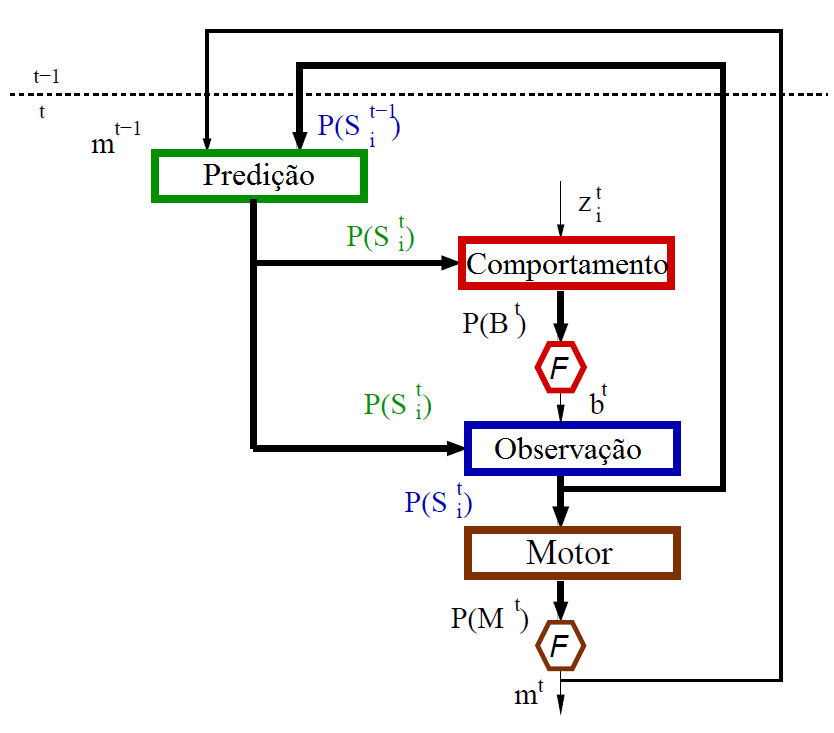
\includegraphics[width=120mm]{images/modelo_probabilistico-carla}
    \caption{\label{img:ModeloProbabilisticoCarla}Modelo Probabilístico de Seleção de Comportamento. Fonte: \cite{INCA2005} [Trocar por tese da Carla]}
\end{figure}

\subsection{Predição}

Nessa etapa, a partir da ação escolhida no período anterior de tempo, se faz uma estimativa de qual será o estado após sua execução.




\subsection{Escolha de comportamento}

Essa etapa é onde a escolha do comportamento acontece. Primeiro se calcula a probabilidade à seguir para cada comportamento .



Depois, se escolhe um comportamento a partir dessas probabilidades calculadas, sendo o escolhido o com a maior probabilidade.

\subsection{Observação}

Tendo, agora, um dos comportamentos escolhido, se atualiza o belief state do agente a partir dos sensores presentes no robô.



\subsection{Escolha de ação motor}

Por último se faz a seleção de uma ação a ser executada pelo robô de forma análoga à seleção de comportamentos. Calcula-se as probabilidade de se executar cada ação  e se escolhe a com maior valor.

\begin{equation}
    P \left( \right)
    P \left( M^t \mid z_i^{0: t} b^{0: t} m^{0: t-1} \lambda_i^{0: t} \beta_i^{0: t} \pi_i \right) \propto \sum\limits_{S_i^{t-1}}
        \left(
            \begin{array}{l}
                P \left( M^t \mid \pi_i \right) x   P \left( \lambda_i^t \mid M^t S_i^t b^t m^{t-1} \pi_i \right)\\
                \times P \left( S_i^t \mid z_i^{0: t} b^{0: t} m^{0: t-1} \lambda_i^{0: t-1} \beta_i^{0: t} \pi_i \right)
            \end{array}
        \right)
\end{equation}


\section{MDP (Processo de Decisão de Markov)}

\section{Diferença Temporal}

\section{Q Learning}

O conjunto dos números complexos, $\mathbb{C}$, representa a segunda
dimensão com coeficientes reais, $\mathbb{R}^{2}$. Os quatérnions
ordinários foram introduzidos por Hamilton em 1843 \cite{book:hamilton:1969}.
Uma maneira é entendê-los como a expansão de $\mathbb{C}$ para a
quarta dimensão com coeficientes reais, $\mathbb{R}^{4}$. Eles são
definidos como:

\begin{equation}
\quat q=\: a\mathbf{1\:+\:}b\mathbf{i\:+\:}c\mathbf{j\:+\:}d\mathbf{k},\label{eq:DefinicaoQuaternion}
\end{equation}
em que a, b, c e d $\in$ $\mathbb{R}$, e \textbf{1},\textbf{ i},\textbf{
j }e\textbf{ k} são os quatro vetores unitários de um sistema com
quatro dimensões

\[
\mathbf{1}=\begin{pmatrix}1 & 0 & 0 & 0\end{pmatrix}^{T},
\]


\[
\mathbf{i}=\begin{pmatrix}0 & 1 & 0 & 0\end{pmatrix}^{T},
\]


\[
\mathbf{j}=\begin{pmatrix}0 & 0 & 1 & 0\end{pmatrix}^{T}
\]
e

\[
\mathbf{k}=\begin{pmatrix}0 & 0 & 0 & 1\end{pmatrix}^{T}.
\]


O $\mathbf{1}$ pode ser omitido nas representações, $\mathbf{1}a=a$.

Um quatérnion ordinário também pode ser definido como 
\begin{equation}
\quat q=(e,\vect v),\label{eq:DefinicaoParQ}
\end{equation}
em que $e$ é a parte escalar e \textbf{$\vect v$} é um vetor de
três dimensões que representa a parte vetorial de $\quat q$. Comparando
com (\ref{eq:DefinicaoQuaternion}), temos

\[
e=a
\]
e

\[
\vect v=\begin{pmatrix}b & c & d\end{pmatrix}^{T}.
\]


A operação entre quatérnions e matrizes é muito utilizada na descrição
de movimentações de corpos rígidos. Sendo assim, uma outra definição
útil para o quatérnion é uma tétrade na forma

\begin{equation}
\mathbf{\quat q}=\begin{pmatrix}a & b & c & d\end{pmatrix}^{T}\label{eq:DefinicaoTetradeQ}
\end{equation}
ou

\begin{equation}
\mathbf{\quat q}=\begin{pmatrix}a\\
b\\
c\\
d
\end{pmatrix}.
\end{equation}


O conjunto de todos os quatérnions ordinários é definido como $\mathbb{H}$,
então \textbf{$\quat q$} $\in$ $\mathbb{H}$.

As regras de multiplicação entre os vetores unitários $\quat 1$,
$\quat i$, $\quat j$ e $\quat k$ não são comutativas e podem ser
vistas a seguir:

\[
\mathbf{i}^{2}=\mathbf{j}^{2}=\mathbf{k}^{2}=-\mathbf{1},
\]
\[
\mathbf{ij}=-\mathbf{ji}=\mathbf{k},
\]
\[
\mathbf{jk}=-\mathbf{kj}=\mathbf{i},
\]
e
\[
\mathbf{ki}=-\mathbf{ki}=\mathbf{j}.
\]


A adição entre quatérnions é definida como
\begin{equation}
\mathbf{\quat q}_{1}+\quat q_{2}=(a_{1}+a_{2})\mathbf{+}(b_{1}+b_{2})\mathbf{i+}(c_{1}+c_{2})\mathbf{j+}(d_{1}+d_{2})\mathbf{k}.\label{eq:DefinicaoSomaQ}
\end{equation}


A subtração entre quatérnions segue o mesmo padrão e é definida como

\begin{equation}
\mathbf{\quat q}_{1}-\quat q_{2}=(a_{1}-a_{2})\mathbf{+}(b_{1}-b_{2})\mathbf{i+}(c_{1}-c_{2})\mathbf{j+}(d_{1}-d_{2})\mathbf{k}.
\end{equation}


Podemos ver, então, que o elemento neutro da adição entre quatérnions
é 

\begin{equation}
\quat q=(\begin{array}{cccc}
0 & 0 & 0 & 0\end{array})^{T}.
\end{equation}


A multiplicação por escalar é definida como

\begin{equation}
A.\quat q_{1}=(A.a_{1})\mathbf{+}(A.b_{1})\mathbf{i+}(A.c_{1})\mathbf{j+}(A.d_{1})\mathbf{k}.\label{eq:DefinicaoMultiplicacaoPorEscalarQ}
\end{equation}


A multiplicação ``$.$'' entre quatérnions é realizada como se realiza
um produto vetorial entre números complexos:

\begin{equation}
\quat q_{1}\quat q_{2}=(a_{1}\mathbf{+}b_{1}\mathbf{i+}c_{1}\mathbf{j+}d_{1}\mathbf{k})(a_{2}+b_{2}\mathbf{i+}c_{2}\mathbf{j+}d_{2}\mathbf{k}).\label{eq:DefinicaoMultiplicacaoQ}
\end{equation}


Podemos omitir ``$.$'' sem perda de significado. O produto escalar
convencional como em $\mathbb{C}$, que mapearia $\mathbb{H}$ em
$\mathbb{R}$ não é usado nesse trabalho.

Realizando a operação distributiva e usando as regras de multiplicação
entre os vetores unitários já citadas anteriormente, obtemos

\begin{equation}
\mathbf{\quat q}_{1}.\mathbf{\quat q}_{2}=\begin{array}{c}
(a_{1}a_{2}-b_{1}b_{2}-c_{1}c_{2}-d_{1}d_{2})+\\
\quat i(a_{1}b_{2}+ba_{2}-c_{1}d_{2}+d_{1}c_{2})+\\
\quat j(a_{1}c_{2}+b_{1}d_{2}+c_{1}a_{2}-d_{1}b_{2})+\\
\quat k(a_{1}d_{2}-b_{1}c_{2}+cb_{2}+d_{1}a_{2}),
\end{array}\label{eq:DefinicaoInicialMultiplicacaoQ}
\end{equation}
em que ``.'' define uma multiplicação escalar.

A partir desses resultados, podemos perceber, sem muitos problemas,
que a multiplicação entre quatérnions é associativa,
\begin{equation}
(\quat q_{1}.\quat q_{2}).\quat q_{3}=\quat q_{1}.(\quat q_{2}.\quat q_{3}),
\end{equation}
distributiva, 
\begin{equation}
(\quat q_{1}+\quat q_{2})\quat q_{3}=\quat q_{1}.\quat q_{3}+\quat q_{2}.\quat q_{3},
\end{equation}
mas não é comutativa. Em geral
\begin{equation}
\quat q_{1}.\quat q_{2}\neq\quat q_{2}.\quat q_{1}.
\end{equation}


O elemento neutro da multiplicação entre quatérnions é

\begin{equation}
\quat q=(\begin{array}{cccc}
1 & 0 & 0 & 0\end{array})^{T}.
\end{equation}


O elemento neutro da adição é absorvente na multiplicação:
\begin{equation}
\quat q_{1}.\begin{pmatrix}0\\
0\\
0\\
0
\end{pmatrix}=\begin{pmatrix}0\\
0\\
0\\
0
\end{pmatrix}.\quat q_{1}=\begin{pmatrix}0\\
0\\
0\\
0
\end{pmatrix}.
\end{equation}


O conjugado de Hamilton de um quatérnion ordinário $\quat q$ é definido
como

\begin{equation}
\mathbf{\quat q^{*}=}a-(b\mathbf{i}+c\mathbf{j}+d\mathbf{k}),\label{eq:DefinicaoConjugadoQ}
\end{equation}
ou, na forma descrita em (\ref{eq:DefinicaoParQ}),

\begin{equation}
\mathbf{\quat q^{*}=}(e,-\vect v).
\end{equation}


A norma de um quatérnion ordinário é definida como

\begin{equation}
\norm{\quat q}=\sqrt{\quat q.\quat q^{*}}=\sqrt{a^{2}+b^{2}+c^{2}+d^{2}}.\label{eq:DefinicaoNormaQ}
\end{equation}


\begin{table}[h]
\begin{longtable}{>{\centering}p{5cm}|>{\centering}p{5cm}}
\hline 
Matriz de Rotação & \selectlanguage{english}%
\hspace{0pt}\foreignlanguage{brazil}{ Uso de nove parâmetros quando
o mínimo necessário são três.}\selectlanguage{brazil}%
\tabularnewline
\hline 
Ângulos de Euler & \selectlanguage{english}%
\hspace{0pt}\foreignlanguage{brazil}{ Degeneração da representação
(falha em representar a transformação) em alguns ângulos.}\selectlanguage{brazil}%
\tabularnewline
\hline 
Ângulo e Eixo & \selectlanguage{english}%
\hspace{0pt}\foreignlanguage{brazil}{ Problemas de unicidade: uma
rotação $\theta$ em torno de um eixo $\vect r$ resulta em uma representação
diferente de uma rotação $-\theta$ em torno de um eixo $-\vect r$.
Uso de quatro parâmetros.}\selectlanguage{brazil}%
\tabularnewline
\hline 
Quatérnion Unitário & \selectlanguage{english}%
\hspace{0pt}\foreignlanguage{brazil}{ Uso de quatro parâmetros}\selectlanguage{brazil}%
\tabularnewline
\end{longtable}

\caption{\label{tab:DesvantagensRepresentacoesRotacao}Tabela multilinha exemplo
sem relação nenhuma com o texto.}
\end{table}



\subsubsection{A Jacobiana Analítica Usando Quatérnions Duais\label{sub:SchunkRBJacobianaAnalitica}}

A Jacobiana Analítica, $\jacob_{a}$, nos dá a relação entre a variação
das variáveis de junta em relação ao tempo e a variação dos termos
do quatérnion dual que representa a pose da ferramenta em relação
ao tempo:
\begin{equation}
\dot{\dq p}_{fer}=\begin{pmatrix}\dot{a_{p}}\\
\dot{b_{p}}\\
\dot{c_{p}}\\
\dot{d_{p}}\\
\dot{a_{d}}\\
\dot{b_{d}}\\
\dot{c_{d}}\\
\dot{d_{d}}
\end{pmatrix}=\begin{pmatrix}\frac{\partial a_{p}}{\partial\theta_{1}} & \frac{\partial a_{p}}{\partial\theta_{2}} & \cdots & \frac{\partial a_{p}}{\partial\theta_{n}}\\
\frac{\partial b_{b}}{\partial\theta_{1}} & \frac{\partial b_{b}}{\partial\theta_{2}} & \cdots & \frac{\partial b_{b}}{\partial\theta_{n}}\\
\vdots & \vdots & \cdots & \vdots\\
\frac{\partial d_{d}}{\partial\theta_{1}} & \frac{\partial d_{d}}{\partial\theta_{2}} & \cdots & \frac{\partial d_{d}}{\partial\theta_{n}}
\end{pmatrix}.\begin{pmatrix}\frac{\partial\theta_{1}}{\partial t}\\
\frac{\partial\theta_{2}}{\partial t}\\
\vdots\\
\frac{\partial\theta_{n}}{\partial t}
\end{pmatrix},
\end{equation}
em que 
\begin{equation}
J_{a}=\begin{pmatrix}\frac{\partial a_{p}}{\partial\theta_{1}} & \frac{\partial a_{p}}{\partial\theta_{2}} & \cdots & \frac{\partial a_{p}}{\partial\theta_{n}}\\
\frac{\partial b_{b}}{\partial\theta_{1}} & \frac{\partial b_{b}}{\partial\theta_{2}} & \cdots & \frac{\partial b_{b}}{\partial\theta_{n}}\\
\vdots & \vdots & \cdots & \vdots\\
\frac{\partial d_{d}}{\partial\theta_{1}} & \frac{\partial d_{d}}{\partial\theta_{2}} & \cdots & \frac{\partial d_{d}}{\partial\theta_{n}}
\end{pmatrix}.
\end{equation}


A Jacobiana de Orientação, $\jacob_{o}$, é constituída pelas quatro
primeiras linhas de $\jacob_{a}$.

O cálculo de $\jacob_{a}$ não é trivial e e é descrito precisamente
em \cite{Adorno2011}. Sua utilização é muito útil para o Modelo Cinemático
Inverso.


\subsubsection{A Jacobiana Geométrica Usando Quatérnions Duais\label{sub:SchunkRBJacobianaGeometrica}}

Há mais de uma maneira de realizar o cálculo da Jacobiana Geométrica,
$\jacob_{g}$. Em uma das maneiras, que segue a maneira de cálculo
usado em \cite{book:siciliano:2009}, obtemos, geometricamente, a
interferência em $\dot{\pose{ref}{fer}}$ causada pela variação de
cada uma das variáveis de junta, separadamente, do manipulador. Essa
relação nos dará a velocidade linear $\vect v_{fer}^{ref}=\begin{pmatrix}v_{x-fer}^{ref} & v_{y-fer}^{ref} & v_{z-fer}^{ref}\end{pmatrix}^{T}$
e também a velocidade angular $\vect{\omega}_{fer}^{ref}=\begin{pmatrix}\omega_{x-fer}^{ref} & \omega_{y-fer}^{ref} & \omega_{z-fer}^{ref}\end{pmatrix}^{T}$;
todas essas, claro, em relação à referência. Ela será na seguinte
forma:
\begin{equation}
\begin{pmatrix}\vect v_{fer}^{ref}\\
\vect{\omega}_{fer}^{ref}
\end{pmatrix}=\jacob_{g}.\dot{\vect{\theta}}.
\end{equation}


Expandindo a equação, temos:

\begin{equation}
\begin{pmatrix}\vect v_{fer}^{ref}\\
\vect w_{fer}^{ref}
\end{pmatrix}=\begin{pmatrix}\frac{\partial x}{\partial\theta_{1}} & \frac{\partial x}{\partial\theta_{2}} & \cdots & \frac{\partial x}{\partial\theta_{n}}\\
\frac{\partial y}{\partial\theta_{1}} & \frac{\partial y}{\partial\theta_{2}} & \cdots & \frac{\partial y}{\partial\theta_{n}}\\
\frac{\partial z}{\partial\theta_{1}} & \frac{\partial z}{\partial\theta_{2}} & \cdots & \frac{\partial z}{\partial\theta_{n}}\\
\frac{\partial\phi_{x}}{\partial\theta_{1}} & \frac{\partial\phi_{x}}{\partial\theta_{2}} & \cdots & \frac{\partial\phi_{x}}{\partial\theta_{n}}\\
\frac{\partial\phi_{y}}{\partial\theta_{1}} & \frac{\partial\phi_{y}}{\partial\theta_{2}} & \cdots & \frac{\partial\phi_{y}}{\partial\theta_{n}}\\
\frac{\partial\phi_{z}}{\partial\theta_{1}} & \frac{\partial\phi_{z}}{\partial\theta_{2}} & \cdots & \frac{\partial\phi_{z}}{\partial\theta_{n}}
\end{pmatrix}.\begin{pmatrix}\frac{\partial\theta_{1}}{\partial t}\\
\frac{\partial\theta_{2}}{\partial t}\\
\vdots\\
\frac{\partial\theta_{n}}{\partial t}
\end{pmatrix},
\end{equation}
em que $\phi_{x}$, $\phi_{y}$ e $\phi_{z}$ são os ângulos de rotação
em torno dos eixos $x$, $y$ e $z$ da ferramenta em relação à referência,
respectivamente.

A maneira desenvolvida diretamente para o cálculo da $J_{g}$ no espaço
dos quatérnions duais pode ser vista em \cite{Adorno2011}.


\section{Desenvolvimento em Tempo Real Rígido\textit{ }usando $\ambiente$%
\footnote{Essa seção faz referência apenas ao trabalho realizado com o $\rhino$,
o $\schu$ usou outro sistema operacional.%
}\label{sub:Linux}}

Para a aplicação desejada, isto é, controle de inserção de agulha
em um paciente, trabalhamos com uma tarefa de altíssima importância,
onde erros na velocidade de execução de um algoritmo ou no seu resultado
lógico podem resultar em danos irreparáveis ao paciente, o que define
a necessidade de computação em tempo real. 

Computação em tempo real não necessariamente implica em uma computação
rápida, mas na garantia de uma resposta em tempo determinístico do
sistema em resposta aos eventos externos. No nosso caso, os eventos
externos serão o eventos que programamos para o manipulador e a realimentação
necessária para o controle. Além de se classificar como sistema de
tempo real, podemos dizer que o tipo de controle esperado reside na
categoria de sistema de tempo real rígido \textit{(hard realtime)}
\cite{NimalNissanke1997}, onde a exatidão no tempo é criticamente
importante e não pode ser sacrificada por outros ganhos. Erros no
controle do tempo das tarefas pode implicar na realização de rotas
indesejáveis pela agulha.

Dada essa necessidade, o sistema operacional escolhido para o desenvolvimento
com o $\rhino$ foi o Ubuntu 9.10, com o Kernel Xenomai 2.6.34.

O desenvolvimento do Xenomai%
\footnote{http://www.xenomai.org/index.php/Main\_Page%
} começou em 2001. Ele é uma base, de código fonte aberto, para desenvolvimento
em tempo real que coopera com o Kernel do Linux, permitindo capacidades
de tempo real rígido a aplicações que executam no espaço do usuário,
com integração praticamente invisível ao ambiente GNU/Linux.

Dentre suas vantagens está a extensa documentação, com suporte rápido
e direto com seus desenvolvedores por meio de lista aberta de e-mails,
e bibliotecas escritas em linguagem C com altíssima padronização e
cuidado. Dentre suas desvantagens está a complexidade de configuração
inicial e a necessidade de um certo conhecimento no funcionamento
em baixo nível do Linux para requisição e compreensão do suporte dado
pelos desenvolvedores e, dada a extensão da documentação, não é incomum
que descrição do funcionamento de uma determinada função ou exemplo
esteja incorreta ou incompleta.

Para realizar a compilação do Xenomai para nossas necessidades, seguimos
os passos descritos pelo corpo do LARA%
\footnote{Pode ser encontrado no site:

http://www.lara.unb.br/wiki/index.php/Ubuntu\_Real-time\_Xenomai%
}, com uma pequena modificação. Além do descrito na referência citada,
adicionamos à compilação a opção para habilitar suporte à interrupções
no espaço do usuário. Para isso, deve-se adicionar à compilação a
seguinte opção:
\begin{itemize}
\item CONFIG\_XENO\_OPT\_NATIVE\_INTR = Enable.
\end{itemize}
Essa opção permite que as interrupções sejam reconhecidas no espaço
de usuário e não somente no espaço de Kernel. 

É importante saber que programas novos desenvolvidos usando o mesmo
ambiente devem evitar essa configuração: ela está agendada para ser
retirada nas futuras versões do Xenomai e seu uso impede o uso de
\textit{debuggers} como o gdb, por exemplo. Os desenvolvedores recomendam
a criação de um \textit{driver} RTDM para o recebimento de interrupções.%
\footnote{Essa discussão que iniciamos pode ser vista em https://mail.gna.org/public/xenomai-help/2010-08/msg00003.html%
}Apesar disso, o nosso objetivo com o uso de interrupções foi apenas
realizar a contagem de pulsos dos \textit{encoders}. Sendo assim,
o suporte para a interrupção como desejamos não justificaria o trabalho
de desenvolvimento de um \textit{driver} RTDM, que é uma tarefa de
desenvolvimento de baixíssimo nível, envolvendo criação de módulos
para o Linux. Isso requereria uma quantidade muito grande de aprofundamento,
estudo no funcionamento básico do $\ambiente$, tempo e, consequentemente,
perda de foco no objetivo maior do uso do $\ambiente$: a criação
do sistema de controle para o $\rhino$.
